%! Author = zlapik
%! Date = 01/04/2023
% Help
% \cmd[option]{arguments}

% Preamble
\documentclass[8pt, landscape]{article}

% Packages
\usepackage{lmodern}
\usepackage[T1]{fontenc}
\usepackage{amsmath}
\usepackage{physics}
\usepackage{amsfonts}
\usepackage{amssymb}
\usepackage{amsthm}
\usepackage{graphicx}
\usepackage{hyperref}
\usepackage{cleveref}
\usepackage{dsfont}
\hypersetup{
    colorlinks=true,
    linkcolor=blue,
    filecolor=magenta,
    urlcolor=red,
    citecolor=green,
    pdftitle={Reinforcement Learning Cheatsheet},
}
\usepackage{listings}
\usepackage{mathtools}
\usepackage{multirow}
\usepackage{paralist}
\usepackage[landscape]{geometry}
\usepackage{lipsum}
\usepackage{tikz}
\usepackage{multicol}
\usepackage{pgfplots}
\usepackage{calc}
\usepackage{algorithm2e}
\usepackage{float}
\usepackage[utf8]{inputenc}
\usetikzlibrary{arrows.meta,shadows,positioning}
\usepackage{xcolor}
\usepackage{pagecolor}
\usepackage{etoolbox}

% Macros
\newboolean{darkmode}
\setboolean{darkmode}{true}

% Definitions
\newcommand{\lengthfromedge}{0.5cm}
\newcommand{\textfontsize}{8pt}
\makeatletter
\renewcommand{\section}{\@startsection{section}{1}{0mm}%
{-1ex plus -.5ex minus -.2ex}%
{0.5ex plus .2ex}%x
{\normalfont\large\bfseries}}
\renewcommand{\subsection}{\@startsection{subsection}{2}{0mm}%
{-1explus -.5ex minus -.2ex}%
{0.5ex plus .2ex}%
{\normalfont\normalsize\bfseries}}
\renewcommand{\subsubsection}{\@startsection{subsubsection}{3}{0mm}%
{-1ex plus -.5ex minus -.2ex}%
{1ex plus .2ex}%
{\normalfont\small\bfseries}}
\newcommand\numberthis{\addtocounter{equation}{1}\tag{\theequation}}
\makeatother
\DeclareMathOperator*{\argmax}{arg\,max}
\DeclareMathOperator*{\argmin}{arg\,min}

% Don't print section numbers
%\setcounter{secnumdepth}{0}

% Page setup
\geometry{top=\lengthfromedge,left=\lengthfromedge,right=\lengthfromedge,bottom=\lengthfromedge}
\pagestyle{empty}
\ifthenelse{\boolean{darkmode}} { \pagecolor{black} \color{white} } {}


% Lists
\setlength{\parindent}{0pt}
\setlength{\parskip}{0pt plus 0.5ex}

% Tikz
\tikzset{
    frame/.style={
        rectangle, draw,
%        text width=6em,
        text centered,
        minimum height=3em,drop shadow,fill=white,
        rounded corners,
    },
    line/.style={
        draw, -{Latex},rounded corners=3mm,
    },
    fontscale/.style = {
        font=\relsize{#1}
    },
    block/.style = {
        rectangle,
        draw,
        text width=8em,
        text centered,
        rounded corners,
        minimum height=2.5em
    },
}

% Document
\begin{document}
    \raggedright
    \fontsize{\textfontsize}{\textfontsize}\selectfont

    \begin{multicols}{3}
        % Multicols Setup
        \setlength{\premulticols}{1pt}
        \setlength{\postmulticols}{0.1pt}
        \setlength{\multicolsep}{1pt}
        \setlength{\columnsep}{1pt}

        % Title
        \begin{center}
            \Large{Reinforcement Learning Cheat Sheet} \\
        \end{center}

        \section*{Summary of Notation}
        Math styles:
        \begin{tabular}{ p{0.2\columnwidth} p{0.7\columnwidth} }
            $\mathbb{P}$     & \verb|\mathbb{P}|     \\
            $\mathbf{P}$     & \verb|\mathbf{P}|     \\
            $\mathtt{P}$     & \verb|\mathtt{P}|     \\
            $\mathit{P}$     & \verb|\mathit{P}|     \\
            $\mathcal{P}$    & \verb|\mathcal{P}|    \\
            $\mathfrak{P}$   & \verb|\mathfrak{P}|   \\
            $\mathnormal{P}$ & \verb|\mathnormal{P}| \\
            $\bar{P}$        & \verb|\bar{P}|        \\
            $\hat{P}$        & \verb|\hat{P}|        \\
            $\tilde{P}$      & \verb|\tilde{P}|      \\
            $\vec{P}$        & \verb|\vec{P}|        \\
            $\overline{P}$   & \verb|\overline{P}|   \\
        \end{tabular}

        \begin{tabular}{ p{0.2\columnwidth} p{0.7\columnwidth} }
            $\doteq$                                 & equality relationship that is true by definition                                          \\
            $\approx$                                & approximately equal                                                                       \\
            $\propto$                                & proportional to                                                                           \\
            Pr$\{X=x\}$                              & probability that a random variable X takes on value x                                     \\
            X $\sim$ p                               & random variable X selected from distribution $p(x)\doteq Pr\{X=x\}$                       \\
            $\mathbb{E}[X]$                          & expected value of random variable X, i.e., $\mathbb{E}[X]\doteq \sum_{x}p(x)\cdot x$      \\
            $\argmax_{x} f(x)$                       & $x$ that maximizes $f(x)$                                                                 \\
            $ln x$                                   & natural logarithm of $x$                                                                  \\
            $\mathrm{e}^x$, $\mathrm{exp}(x)$        & the base of the natural logarithm, $e\approx 2.71828$, carried to power $x$, $e^{ln x}=x$ \\
            $\mathbb{R}$                             & set of real numbers                                                                       \\
            $f: \mathcal{X} \rightarrow \mathcal{Y}$ & function f from elements of set $\mathcal{X}$ to elements fo set $\mathcal{Y}$            \\
            $\leftarrow$                             & assignment operator                                                                       \\
            $(a,b]$                                  & interval from $a$ to $b$ including $b$                                                    \\
        \end{tabular}

        \begin{tabular}{ p{0.2\columnwidth} p{0.7\columnwidth} }
            $\epsilon$               & probability of taking a random action in an $\epsilon$-greedy policy                        \\
            $\alpha$, $\beta$        & step-size parameters                                                                        \\
            $\gamma$                 & discount factor                                                                             \\
            $\lambda$                & decay-rare parameter for eligibility traces                                                 \\
            $\mathds{1}_{predicate}$ & indicator function ($\mathds{1}_{predicate}$ $\doteq$ 1 if the $predicate$ is true, else 0) \\
        \end{tabular}


        In a multi-arm bandit problem:
        \begin{tabular}{ p{0.2\columnwidth} p{0.7\columnwidth} }
            $k$          & number of actions(arms)                                           \\
            $t$          & discrete time step or play number                                 \\
            $q_{*}(a)$   & true value (expected reward) of action $a$                        \\
            $Q_{t}(a)$   & estimate at time $t$ of $q_{*}(a)$                                \\
            $N_{t}(a)$   & number if times action $a$ has been selected up prior to time $t$ \\
            $H_{t}(a)$   & learned preference for selecting action $a$ at time $t$           \\
            $\pi_{t}(a)$ & probability of selecting action $a$ at time $t$                   \\
            $\bar{R}_t$  & estimate at time t of the expected reward given $\pi_t$           \\
        \end{tabular}

        In Markov Decision Processes:
        \begin{tabular}{ p{0.2\columnwidth} p{0.7\columnwidth} }
            $s$,$s'$          & states                                                        \\
            $a$               & an actions                                                    \\
            $r$               & a reward                                                      \\
            $\mathcal{S}$     & set of all non-terminal states                                \\
            $\mathcal{S}^{+}$ & set of all states, including terminal states                  \\
            $\mathcal{A}(s)$  & set of all actions in state $s$                               \\
            $\mathcal{R}$     & set of all possible rewards, a finite subset of $\mathbb{R}$  \\
            $\subset$         & subset of; ($\mathcal{R}\subset\mathbb{R}$)                   \\
            $\in$             & is an element of; e.g. ($s\in\mathcal{S}$, $r\in\mathcal{R}$) \\
        \end{tabular}

        \begin{tabular}{ p{0.2\columnwidth} p{0.7\columnwidth} }
            $t$        & discrete time step                                                            \\
            $T, T(t)$  & final time step of an episode, or of the episode oncluding time step $t$      \\
            $A_t$      & action at tim et                                                              \\
            $S_t$      & state at time $t$, typicaly due, stochastically, to $S_{t-1}$ and $A_{t-1}$   \\
            $R_t$      & state at time $t$, typicaly due, stochastically, to $S_{t-1}$ and $A_{t-1}$   \\
            $\pi$      & policy (decision-making-rule)                                                 \\
            $\pi(s)$   & action taken in state $s$ under $deterministic$ policy $\pi$                  \\
            $\pi(a|s)$ & probability of taking action $a$ in state $s$ under $stochastic$ policy $\pi$ \\
        \end{tabular}

        \begin{tabular}{ p{0.2\columnwidth} p{0.7\columnwidth} }
            $G_t$                                    & return following time $t$                                              \\
            $h$                                      & horizon, th etime step one look up to in a forward view                \\
            $G_{t:t+n}$                              & n-ste return from $t+1$ to $t+n$, or to $h$ (discounted and corrected) \\
            $\bar{G}_{t:h}$                          & flat return (undiscounted and uncorrected) from $t+1$ to $h$           \\
            $G_{t}^{\lambda}$                        & $\lambda$-return                                                       \\
            $G_{t:h}^{\lambda}$                      & truncated, corrected $\lambda$-return                                  \\
            $G_{t}^{\lambda s}$, $G_{t}^{\lambda a}$ & $\lambda$-return, corrected by estimate state, or action, values       \\
        \end{tabular}

        \begin{tabular}{ p{0.2\columnwidth} p{0.7\columnwidth} }
            $p(s',r|s,a)$ & probability of transitioning to state $s'$ and receiving reward $r$ when in state $s$ and taking action $a$ \\
            $p(s'|s,a)$   & probability of transitioning to state $s'$ when in state $s$ and taking action $a$                          \\
            $r(s,a)$      & expected reward when in state $s$ and taking action $a$                                                     \\
            $r(s,a,s')$   & expected reward when in state $s$ and taking action $a$, and transitioning to state $s'$                    \\
        \end{tabular}

        \begin{tabular}{ p{0.2\columnwidth} p{0.7\columnwidth} }
            $v_{\pi}(s)$   & value of state $s$ under policy $\pi$ (expected-reward)                \\
            $v_{*}(s)$     & value of state $s$ under the optimal policy                            \\
            $q_{\pi}(s,a)$ & value of state $s$ and action $a$ under policy $\pi$ (expected-reward) \\
            $q_{*}(s,a)$   & value of state $s$ and action $a$ under the optimal policy             \\
        \end{tabular}

        \begin{tabular}{ p{0.2\columnwidth} p{0.7\columnwidth} }
            $V$,$V_t$                  & array estimates of state values function $v_\pi$ or $v_*$                                      \\
            $Q$,$Q_t$                  & array estimates of state-action values function $q_\pi$ or $q_*$                               \\
            $V_t(s)$                   & expected approximate action value; for example, $\bar{V_t}(s)\doteq \sum_{a} \pi(a|a)Q_t(s,a)$ \\
            $U_t$                      & target for estimate at time $t$                                                                \\
            $\delta_t$                 & temporal-difference (TD) error at $t$ (a random varibale)                                      \\
            $\delta_t^s$, $\delta_t^a$ & state-and action-specific forms of the TD error                                                \\
            $n$                        & in n-step methods, n is th enumber of steps of bootstrapping                                   \\
        \end{tabular}

        \begin{tabular}{ p{0.2\columnwidth} p{0.7\columnwidth} }
            $d$                          & dimensionality -- the number of components of                                          \\
            $\vb{w}$, $\vb{w}_t$         & d-vector of weights underlying an approximate value function                           \\
            $w_i$, $w_{t,i}$             & the $i$th component of learnable wright vector $\vb{w}$                                \\
            $v_{\vb{w}}(s)$              & alternate notation for $\hat{v}(s,\vb{w})$                                             \\
            $\hat{q}(s,a,\vb{w})$        & approximate value of state-action pair s,a given weight vector $\vb{w}$                \\
            $\nabla \hat{v}(s,'vb{w})$   & column vector of partial derivatives of $\hat{v}(s,\vb{w})$ with respect to $\vb{w}$   \\
            $\nabla \hat{q}(s,a,\vb{w})$ & column vector of partial derivatives of $\hat{q}(s,a,\vb{w})$ with respect to $\vb{w}$ \\
        \end{tabular}

        \begin{tabular}{ p{0.2\columnwidth} p{0.7\columnwidth} }
            $\vb{x}(s)$          & vector of features visible in state $s$                                                                                  \\
            $\vb{x}(s,a)$        & vector of featres visible when in state $s$ taking action $s$                                                            \\
            $x_i(s)$, $x_i(s,a)$ & the $i$th component of $\vb{x}(s)$ or $\vb{x}(s,a)$                                                                      \\
            $\vb{x}_t$           & short-hand for $\vb{x}(S_t)$ or $\vb{x}(S_t, A_t)$                                                                       \\
            $\vb{w}^\top x$      & inner product of vectors, $\vb{w}^\top x\doteq=\sum_{i}w_i x_i$; for example, $\hat{v}(s,\vb{w})\doteq \vb{w}^\top x(s)$ \\
            $\vb{v}$, $\vb{v}_t$ & secondary $d$-vector of weights, used to learn $\vb{w}$                                                                  \\
            $\vb{z}_t$           & $d$-vector of eligibility traces at tim $t$                                                                              \\
        \end{tabular}

%        \begin{tabular}{ p{0.2\columnwidth} p{0.7\columnwidth} }
%            TODO
%        \end{tabular}
    \end{multicols}

    \newpage

    \begin{multicols}{3}
        \section{Introduction}

        \subsection{Recap}
        foo:
        \begin{equation}
            \mathbb{E}[X] = \sum_{x_i} x_i \cdot Pr\{ X = x_i \}
        \end{equation}
        foo:
        \begin{equation}
            \mathbb{E}[X | Y = y_j] = \sum_{x_i} x_i \cdot Pr\{ X = x_i | Y = y_j\}
        \end{equation}
        foo:
        \begin{equation}
            \mathbb{E}[X | Y = y_j] = \sum_{z_k} Pr\{Z=z_k | Y = y_j\} \cdot \mathbb{E}[X|Y = y_j, Z = z_k]
        \end{equation}
%        $\mathbb{E}[X] \stackrel{.}{=} \sum_{x_i} x_i \cdot Pr\{ X = x_i \}$
%        $\mathbb{E}[X | Y = y_j] = \sum_{x_i} x_i \cdot Pr\{ X = x_i | Y = y_j\}$
%        $\mathbb{E}[X | Y = y_j] = \sum_{z_k} Pr\{Z=z_k | Y = y_j\} \cdot \mathbb{E}[X|Y = y_j, Z = z_k]$


        \section{Multi-armed Bandits}


        \section{Finite Markov Decision Process}

        \subsection{Agent-Environment Interaction}
        \begin{center}
            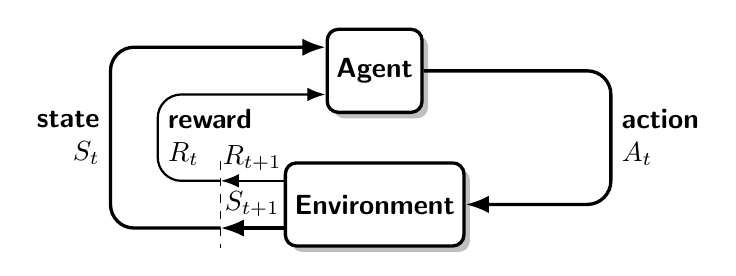
\begin{tikzpicture}[font=\sffamily\bfseries,very thick,node distance = 4cm]
                \node [frame] (agent) {Agent};
                \node [frame, below=0.6cm of agent] (environment) {Environment};
                \draw[line] (agent) -- ++ (3,0) |- (environment)
                node[right,pos=0.25,align=left] {action\\ $A_t$};
                \coordinate[left=8mm of environment] (P);
                \coordinate[above=3mm of environment.west] (ENW);
                \coordinate[below=3mm of environment.west] (ESW);
                \coordinate[above=3mm of agent.west] (ANW);
                \coordinate[below=3mm of agent.west] (ASW);
                \draw[thin,dashed] (P|-environment.north) -- (P|-environment.south);
                \draw[line] (ESW) -- (P |- ESW)
                node[midway,above]{$S_{t+1}$};
                \draw[line,thick] (ENW) -- (P |- ENW)
                node[midway,above]{$R_{t+1}$};
                \draw[line] (P |- ESW) -- ++ (-1.4,0) |- (ANW)
                node[left, pos=0.25, align=right] {state\\ $S_t$};
                \draw[line,thick] (P |- ENW) -- ++ (-0.8,0) |- (ASW)
                node[right,pos=0.25,align=left] {reward\\ $R_t$};
            \end{tikzpicture}
        \end{center}


        \section{Dynamic Programming}


        \section{Monte Carlo Methods}


        \section{Temporal-Difference Learning}


        \section{n-step Bootstrapping}


        \section{Planning and Learning}


        \section{On Policy Prediction with Approximation}


        \section{On Policy Control with Approximation}


        \section{Off Policy Prediction with Approximation}


        \section{Eligibility Traces}


        \section{Policy Gradient Methods}


        \section{Psychology}


        \section{Neuroscience}


        \section{Application and case studies}


        \section{Frontiers}
    \end{multicols}
\end{document}